\documentclass[notes,compress,sanserif,professionalfont]{beamer}
\usetheme{boxes} %Boadilla, Berkeley, Dresden, Rochester, Pittsburgh
\useoutertheme{miniframes} %split, shadow, infolines, default
\usepackage{hyperref}
\usepackage{pxfonts}
\usepackage{amsmath}
\usepackage{amssymb}
\usepackage{amsfonts}
\usepackage{enumerate}
\usepackage{natbib}
\usepackage{xcolor}
\usepackage{multirow}
\usepackage{tikz}
\usepackage{subfigure}
\usetikzlibrary{arrows,shapes}
\beamertemplateballitem % make bullets and items fancy balls
\useheadtemplate{%
\vbox{%
\vskip1pt%
\beamerline{\insertnavigation{\paperwidth}}%
\vskip-5pt
}
}
%\renewcommand{\frametitle}[1]{\begin{center}\textbf{#1}\end{center}}
% Define local notation.

\def\etal{{\emph{et alia\/}}}
\def\sR{\textsf{R}}
\def\argmax{\mathop{\rm argmax}}
\def\cL{{\cal L}}


\begin{document}
\title{Selecting the Optimal Credit Card Portfolio}
\author{Remco A.~Scheepmaker}
\date{10 June 2024}

\begin{frame}
  \titlepage
\end{frame}

% Presentation 1 (June 10): TOPIC AND MOTIVATION. THE PROBLEM. ONLY SHORT: describing the economic model used to structure the answer to the problem. 
% ~30 minutes + 10 minutes discussion.

\section{Introduction}

% Let's apply some Business Analytics to Personal Finance. 
\begin{frame}
    \frametitle{ }
    \begin{quote}
        \centerline{In 30 minutes\ldots}
        \vskip 16pt
        \centerline{you'll know how to be financially sophisticated}
        \centerline{and profit from the financially na\"{i}ve!}
    \end{quote}
\end{frame}

\begin{frame}
    \frametitle{Outline}

    \begin{itemize}
        \item Introduction
        \begin{itemize}
            \item Why credit cards?
            \item The market for credit card rewards
        \end{itemize}

        \item Literature
        \begin{itemize}
            \item Some interesting patterns
        \end{itemize}

        \item \emph{Intermezzo}: credit scores
        \begin{itemize}
            \item Reaching financial sophistication
        \end{itemize}

        \item Optimizing the benefit
        \begin{itemize}
            \item Theory
            \item Empirical Specification
         \end{itemize}

         \item Data
         \begin{itemize}
            \item Credit Cards 
            \item Budgets
        \end{itemize}

        \item Summary \& Conclusions
    \end{itemize}
\end{frame}

\begin{frame}
    \frametitle{Why Credit Cards?}
    \begin{itemize}
        \item I'm a big credit card nerd! 
        \item A unique hobby that \emph{pays} me money:
    \end{itemize}
    \begin{center}
        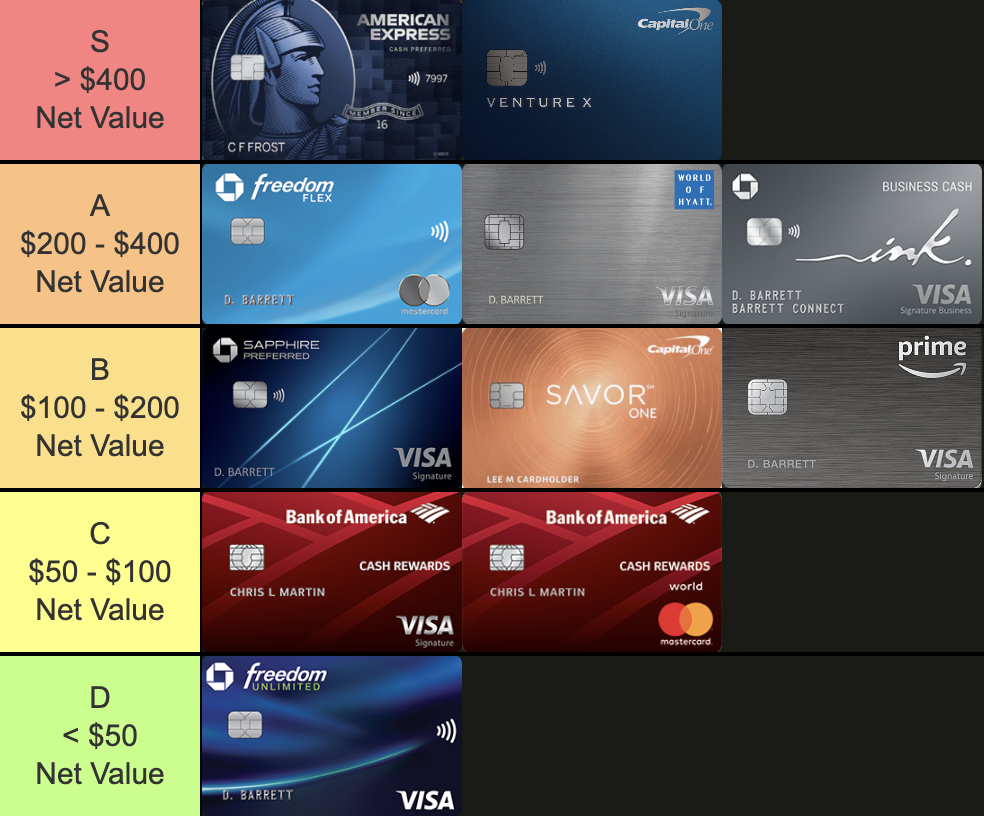
\includegraphics[width=.75\textwidth]{../Misc/Tiermaker_May2024_NetValue.png}
    \end{center}
\end{frame}
    
\begin{frame}
\frametitle{The Market for Credit Cards}
\begin{itemize}
    \item Credit cards are also an important part of the economy
    \begin{itemize}
        \item Consumers spent \$3.2 trillion using credit cards in 2022\footnote{\emph{The consumer credit card market}, \citet{cfpb:2023}}
        \item Total credit card debt passed \$1.1 trillion (82\% revolving)
        \item \$130 billion charged in interest and fees (2022)
    \end{itemize}
    \begin{center}
        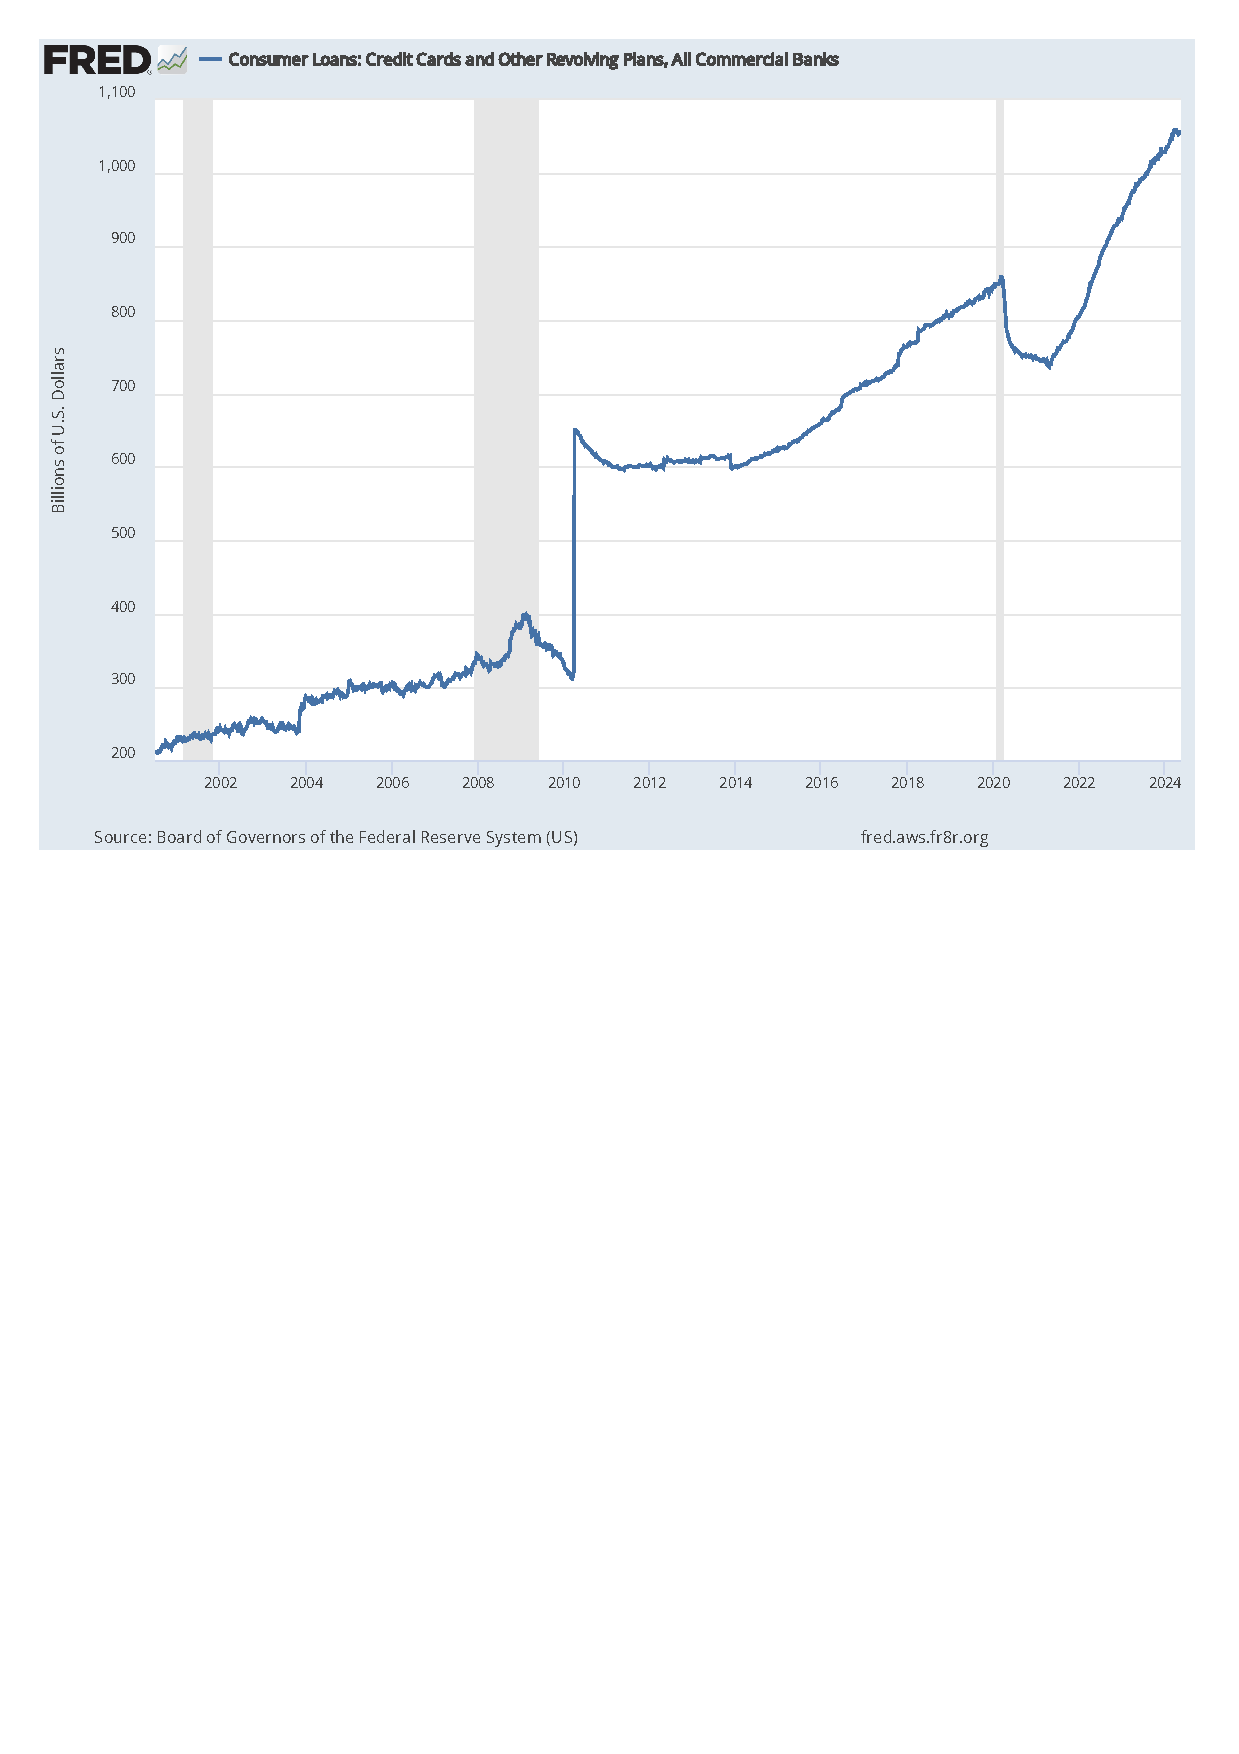
\includegraphics[width=.75\textwidth]{../Misc/FRED_CCDebt.pdf}
    \end{center}
\end{itemize}
\end{frame}

\begin{frame}
    \frametitle{Credit Cards Rewards}
    \begin{itemize}
        \item<+-> Rewards programs can also be beneficial
        \begin{itemize}
            \item Total rewards earned in 2022: $>$\$40 billion\footnote{\emph{The consumer credit card market}, \citet{cfpb:2023}}
            \item The average account redeemed \$167
            \item The average American has 3.9 accounts
        \end{itemize}
        \bigskip
        \item<+-> My project
        \begin{itemize}
            \item How should different consumers optimize their credit card portfolio?
            \item What is the value of this optimal portfolio?
            \item What is the marginal benefit of additional cards?
            \item Is there an optimal number of cards?
        \end{itemize}
    \end{itemize}
\end{frame}
    

% 2. Notwithstanding all the debt, credit cards can also be rewarding.
%     - Explain the economics of credit card transactions.
%     - Interchange fees, processing fees, network fees. See Hayashi 2009!!!
%     - Retailers calculate this into all prices. If you pay cash or debit you subsidize the credit card users who get rewards (average $151 per year).
%     - Reverse Robinhood mechanism: low incomes subsidize high incomes, but this seems to be only partially true: it's mostly low FICO scores who subsidize high FICO scores.


\section{Literature}

\begin{frame}
    \frametitle{The Economics of Credit Card Transactions}
    \begin{itemize}
        \item<+-> First, \emph{who pays for the rewards?}
        \item Example of a \$100 purchase (from F. Hayashi, \citeyear{hayashi:2009}):
    \end{itemize}
    \begin{center}
        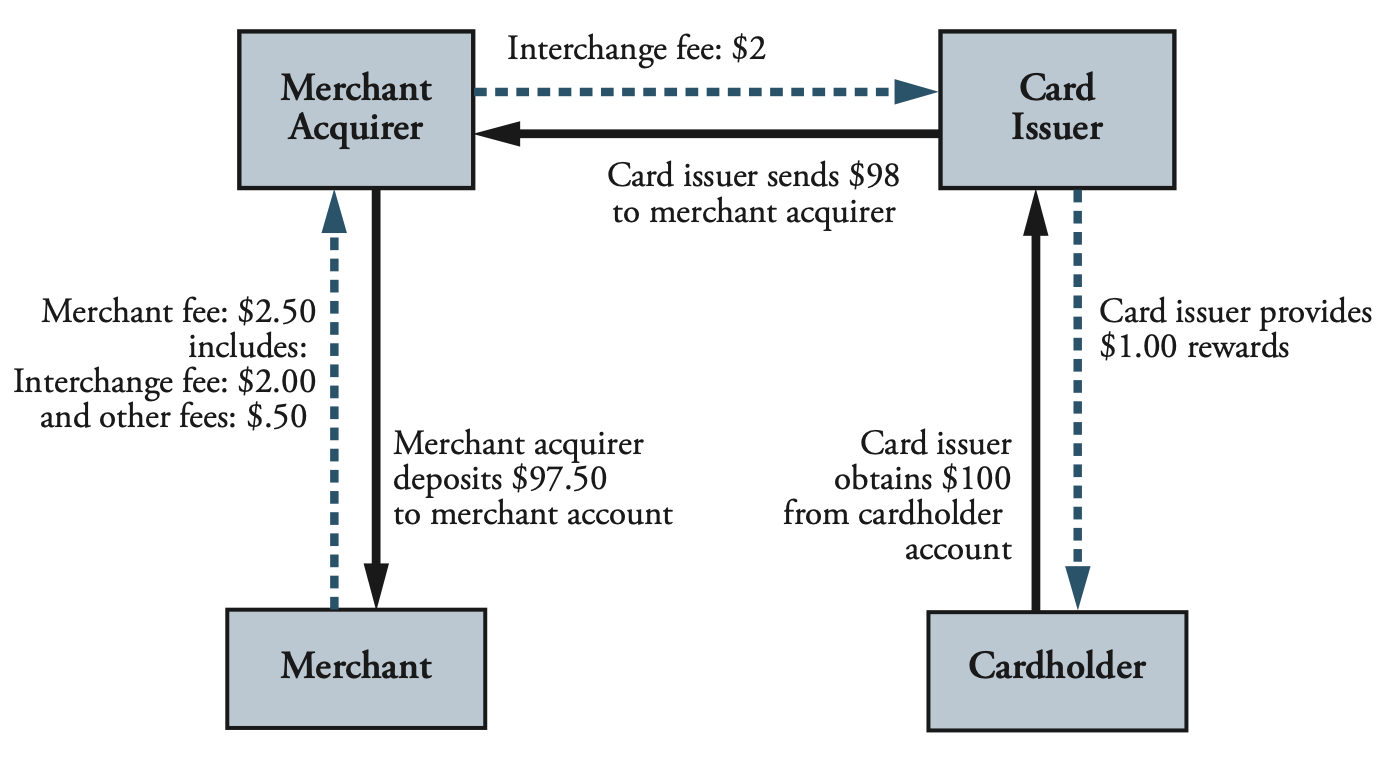
\includegraphics[width=.75\textwidth]{../Misc/Hayashi2009_Fig1.png}
    \end{center}    
    \begin{itemize}
        \item<+-> Merchants likely pass the fees through to \emph{all} customers
        \item<+-> ``Credit card rewards programs, are not likely to be efficient (\ldots) rewards may potentially be too generous,
        lowering overall consumer welfare.''
    \end{itemize}
% providing payment card rewards can maximize efficiency only when
% the merchant’s transactional benefit exceeds the payment service pro-
% viders’ joint net cost of a card transaction.
\end{frame}

\begin{frame}
    \frametitle{The Reverse Robin Hood Mechanism}
    \begin{itemize}
        \item Rewards transfer money from low-income to high-income households (S. Schuh \emph{et al.}, \citeyearpar{schuetal:2010})
    \end{itemize}
    \begin{center}
        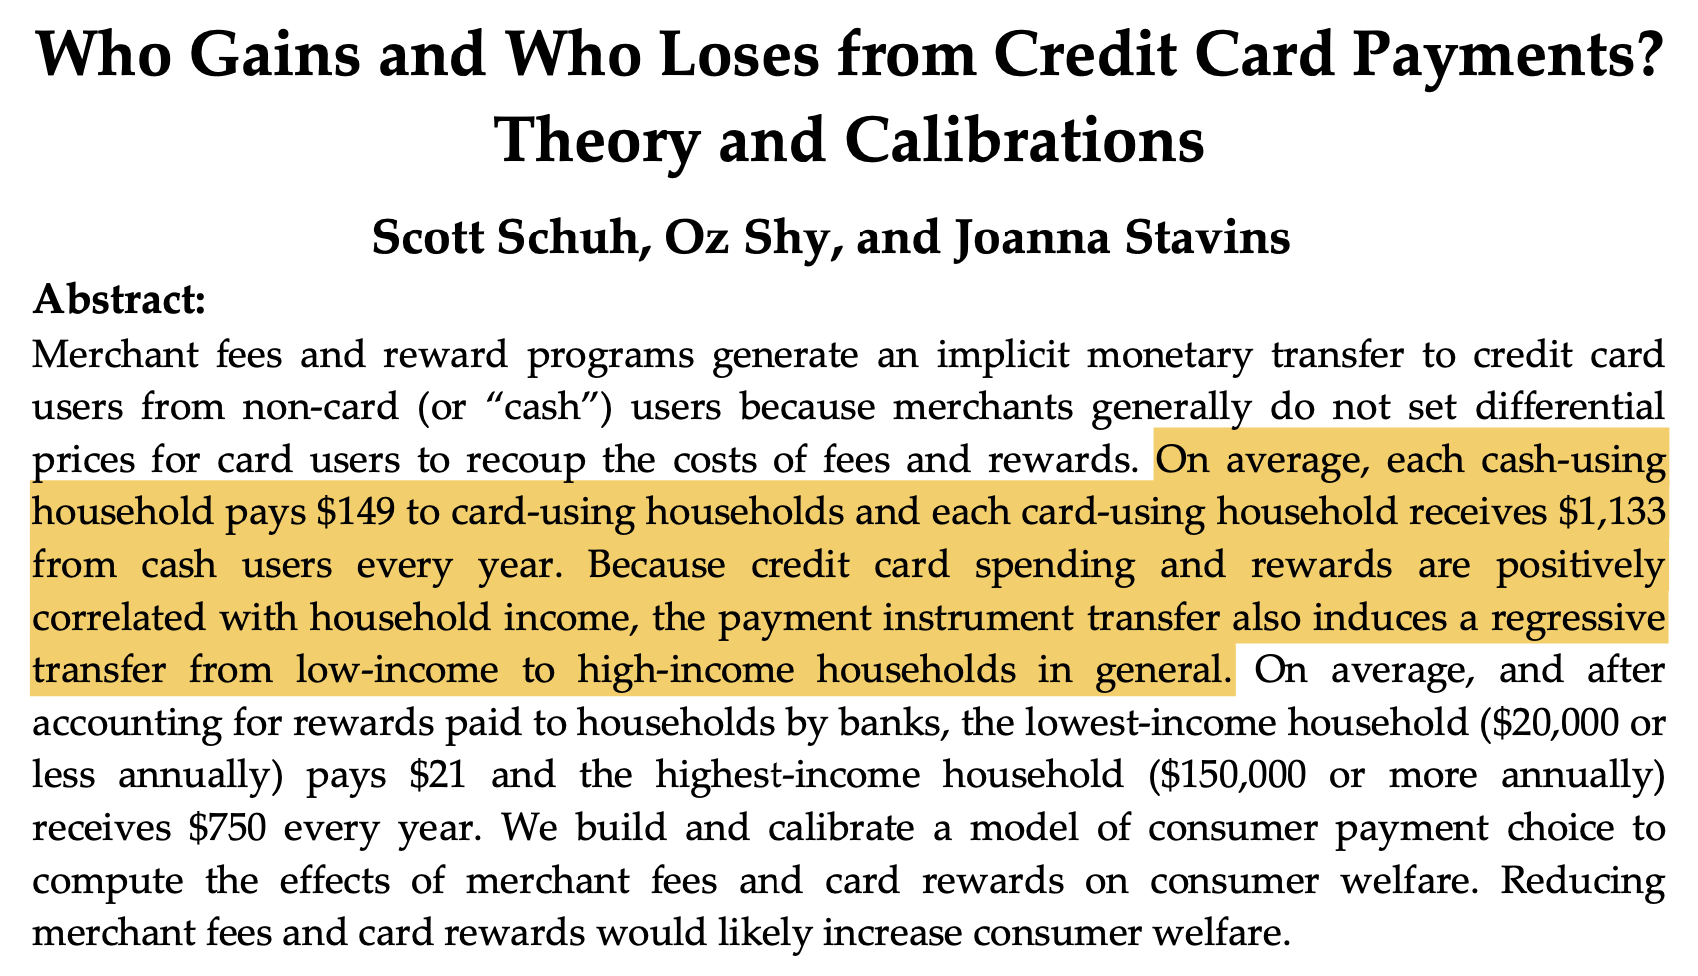
\includegraphics[width=\textwidth]{../Misc/Schuh2010.png}
    \end{center}    
\end{frame}

\begin{frame}
    \frametitle{Financial Sophistication}
    \begin{itemize}
        \item S. Agarwal \emph{et al.}, \citeyearpar{agaretal:2023} show this model is incomplete:
        \begin{itemize}
            \item Redistribution takes place from low to high FICO scores \emph{regardless} of income
            \item High-scoring cardholders benefit primarily at the expense of high-income cardholders with low credit scores
            \item FICO scores are a proxy for \emph{Financial Sophistication}\footnote{The ability of consumers to make informed decisions and avoid mistakes in the use of financial products.}
        \end{itemize}
    \end{itemize}
    \begin{center}
        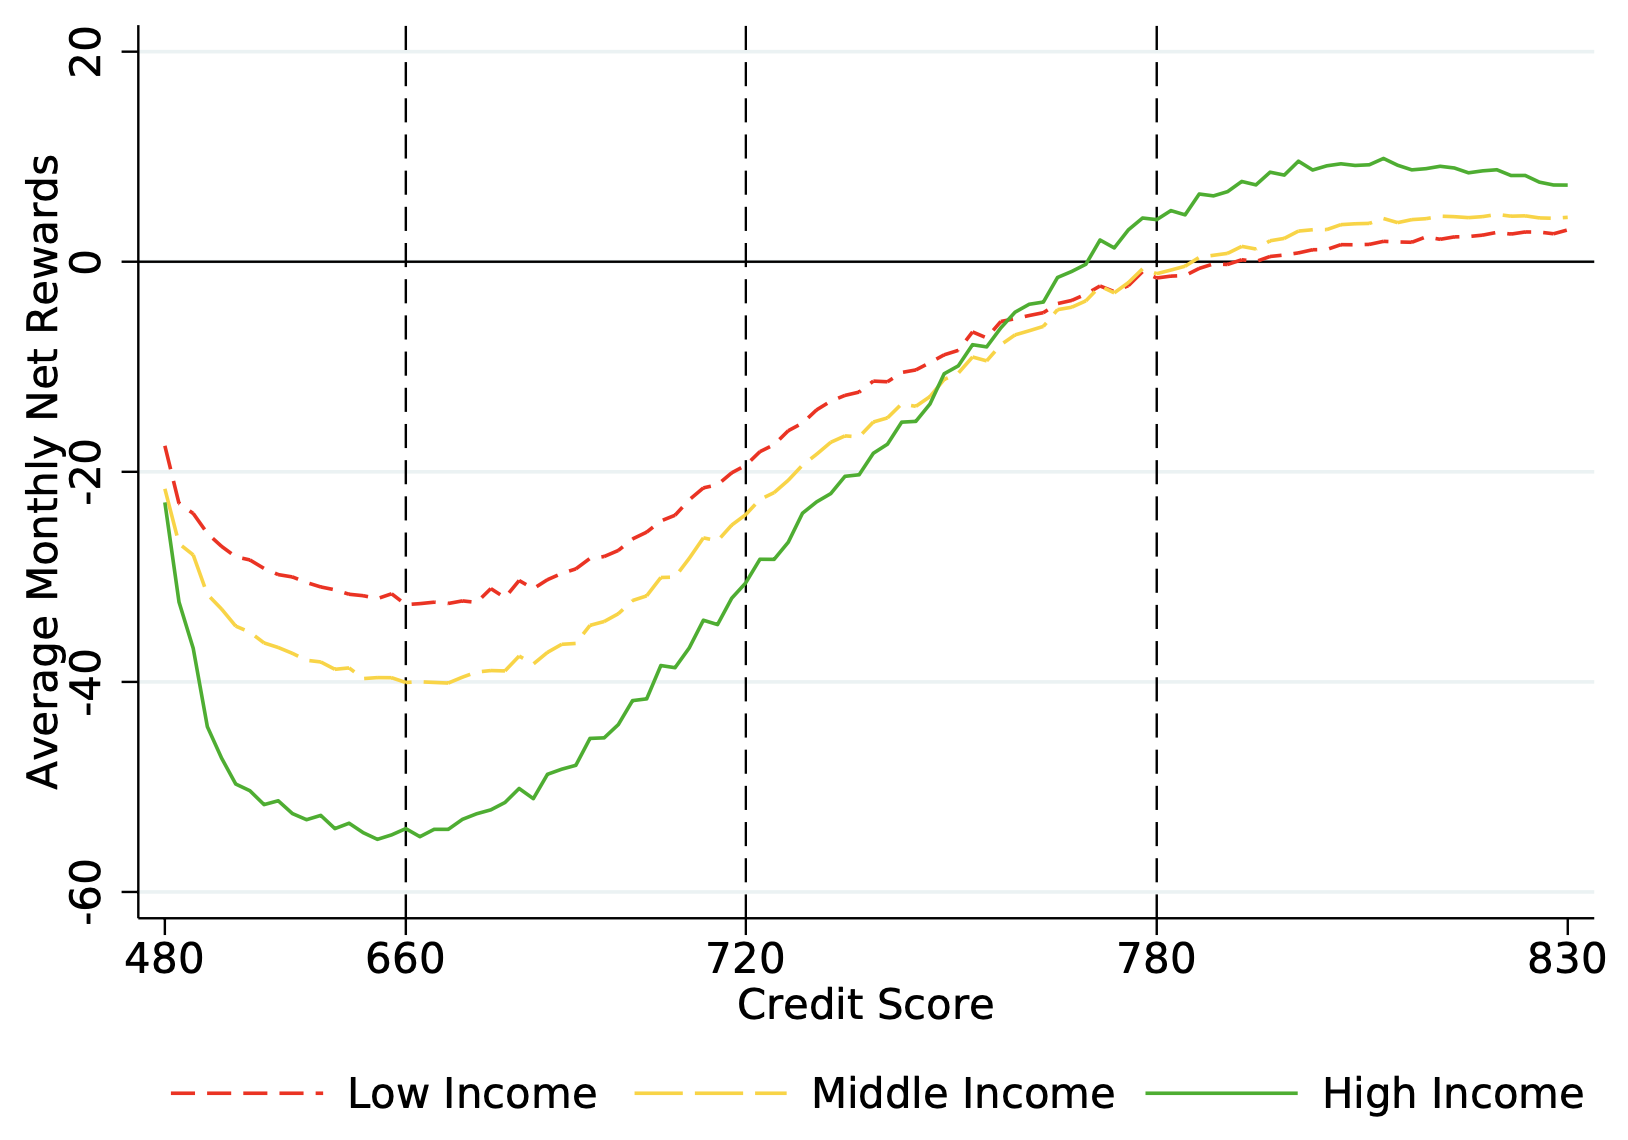
\includegraphics[width=.6\textwidth]{../Misc/Agarwal_NetRewardsByIncome.png}
    \end{center}    
\end{frame}
    
% \begin{frame}
%     \frametitle{ ? }
%     \begin{itemize}
%         \item Banks ?
%     \end{itemize}
%     \begin{center}
%         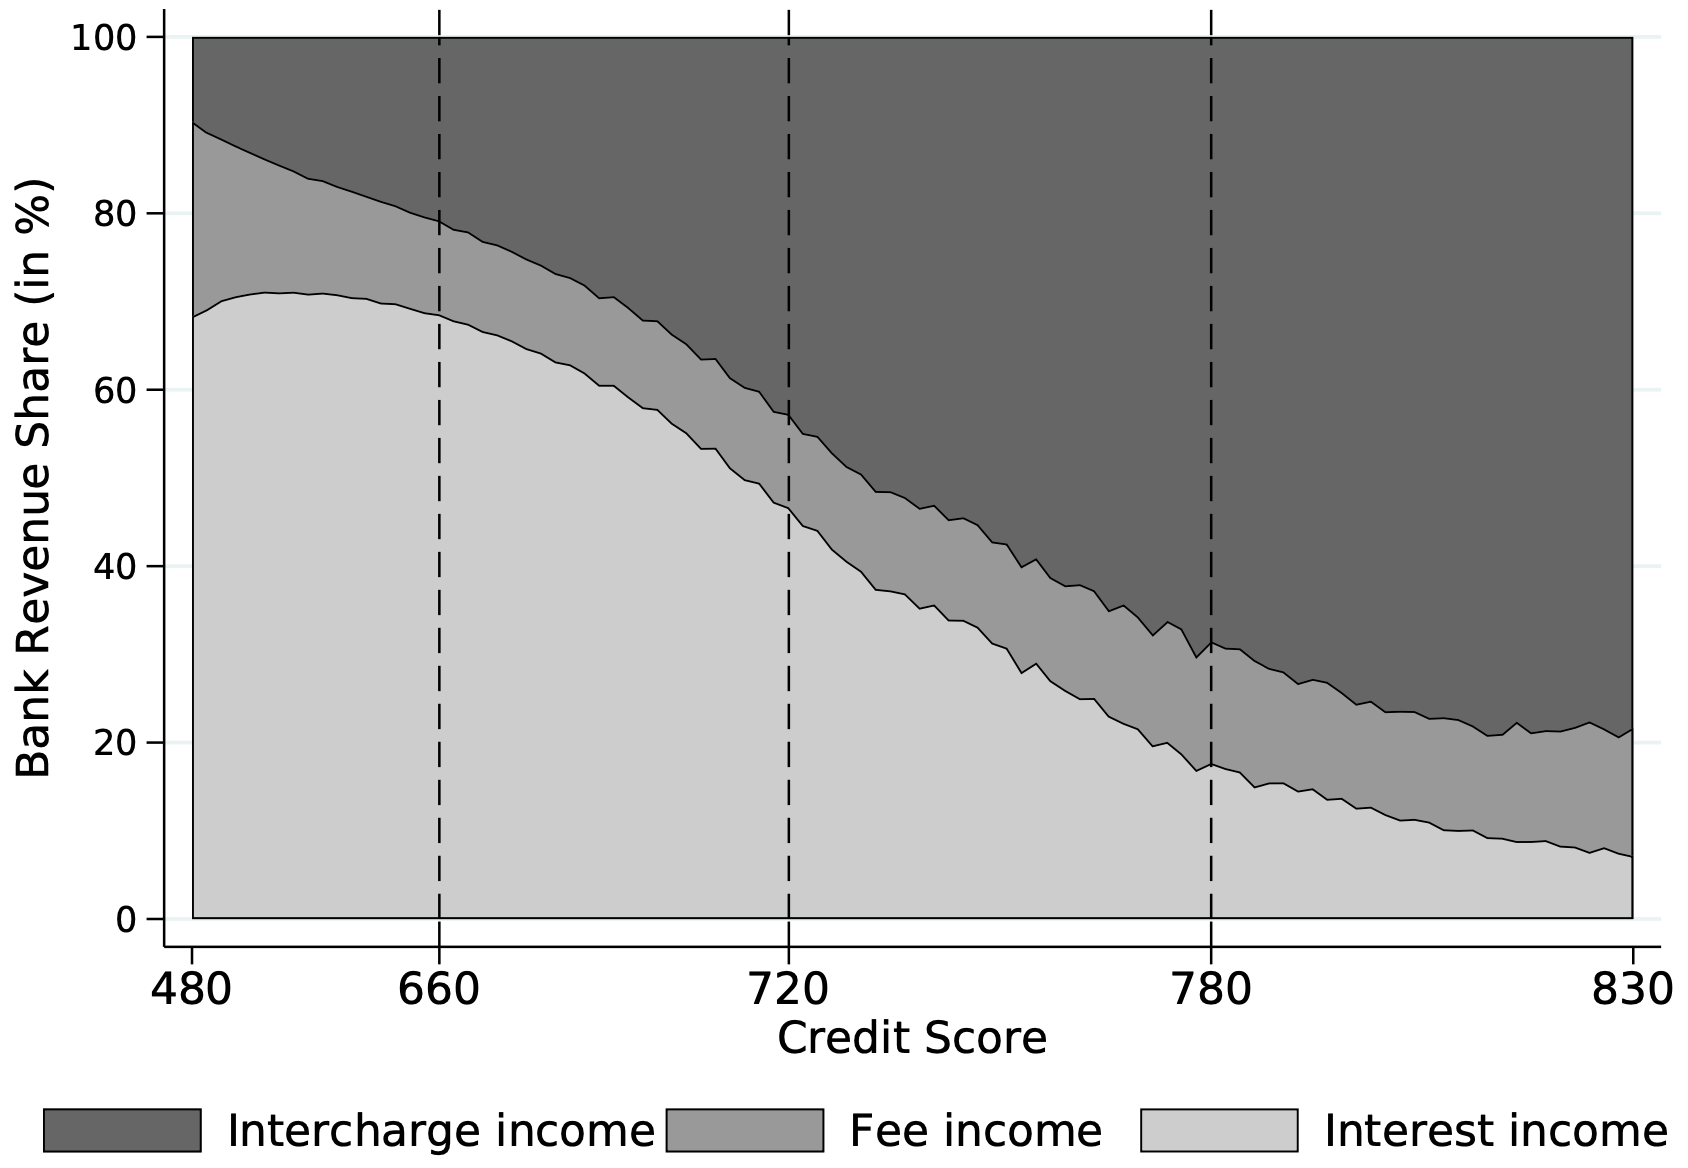
\includegraphics[width=.6\textwidth]{../Misc/Agarwal_BankRevenueShares.png}
%     \end{center}    
% \end{frame}

\begin{frame}
    \frametitle{Literature Summary}
    \begin{itemize}
        \item<+-> Rewards Programs are inefficient
        \begin{itemize}
            \item There likely exists hidden price action
            \item Great! This can be exploited by smart consumers! 
        \end{itemize}
        \bigskip
        \item<+-> Money flows from the na\"{i}ve to the sophisticated
        \begin{itemize}
            \item We need to be financially sophisticated before we can benefit
        \end{itemize}
   \end{itemize}
 \end{frame}


\section{Intermezzo: Credit Scores}

\begin{frame}
    \frametitle{What is a FICO Score?}
    \begin{itemize}
        \item A scoring model used by lenders to estimate consumer risk 
    \end{itemize}
    \begin{center}
        
\includegraphics[width=.75\textwidth]{../Misc/FICOComposition.png}
    \end{center}    
\end{frame}    

\begin{frame}
    \frametitle{What is a FICO Score?}
    \begin{itemize}
        \item Higher scores are less risky and get better terms and credit cards 
    \end{itemize}
    \begin{center}
        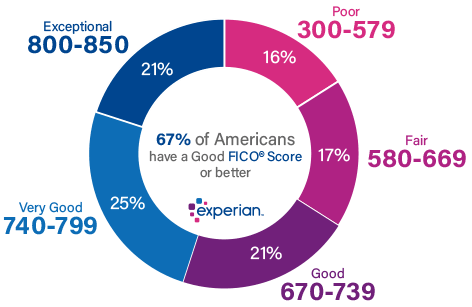
\includegraphics[width=.8\textwidth]{../Misc/FICOExperian.png}
    \end{center}    
\end{frame}    

\begin{frame}
    \frametitle{Smart Financial Habits}
    \begin{itemize}
        \item Only use credit cards if you can pay them off \emph{in full} the next month
        \begin{itemize}
            \item Paying $>$ 20\% APR interest on revolving balances, negates all benefits!
        \end{itemize}
        \item Always pay on time (payment history)
        \item Keep utilization ratio $<$ 10--30\% (amount owed)
        \item Don't apply too often, too quickly (new credit)
        \item Keep your oldest card open forever (length of credit history)
   \end{itemize}
 \end{frame}

 \begin{frame}
    \frametitle{Myth Debunked}
    \begin{itemize}
        \item No, having many cards does \emph{not} ruin your credit score:
    \end{itemize}

    \begin{center}
        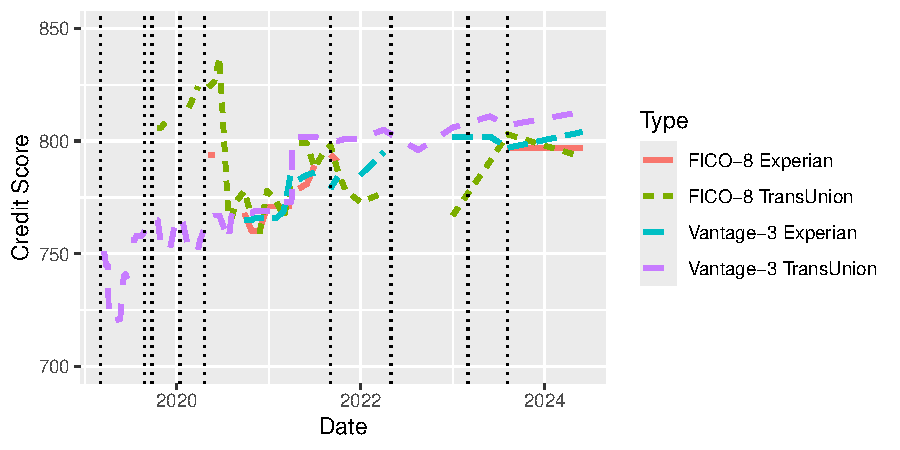
\includegraphics[width=\textwidth]{../Figures/CreditScoresTimeSeries.pdf}
    \end{center}    
\end{frame}    


\section{Optimizing the benefit}

% What does theory say about what type of data to collect?
% What does theory say about the Empirical Specification?
% Check how Schuh modeled stuff? 

% 5. Taking it to the next level.
%     - But how can we optimize this further? 
%     - I will study how to select the optimal credit card portfolio for maximum rewards.
%     - Comparing different heuristics? Optimal vs 1-card vs 
%       something-sub-optimal-most-people-tend-to-do?
%     - Do for different simulated budgets and look for heterogeneity across budgets or 
%       typical users.

% 6. Budgets
%     - Research average spending of americans and change it to 5 typical consumers?
%     - See CFPB Chapter 3! Maybe split consumers by FICO score that correlates with budget?

% 7. Very simple economic model
%     - Y = X*b + benefits - fees, etc.


\begin{frame}
    \frametitle{Theory -- The Problem}
    \begin{itemize}
        \item Credit cards reward the user with spend (cash back or points), but some also have static benefits (lounge access, travel credit, free Disney+, etc.) and annual fees
        \bigskip
        \item To maximize the net benefit, how should a financially sophisticated cardholder optimize her credit card portfolio?
        \bigskip
        \item Credit card data is heavily regulated and very private! We need simulations using realistic input data.
    \end{itemize}
\end{frame}    

\begin{frame}
    \frametitle{Theory -- Dynamic Programming}
    \begin{itemize}
        \item This is a \emph{Dynamic Program}, which ChatGPT defines as:  
        \begin{itemize}
            \item ``A method or algorithm designed to solve problems by breaking them down into {\bf simpler subproblems}, solving each of those subproblems just once, and {\bf storing their solutions}. The key idea is to use past computations to avoid redundant work, which makes the approach efficient. This technique is especially useful for optimization problems where a solution can be constructed incrementally from solutions to subproblems.''
        \end{itemize}    
    \end{itemize}
\end{frame}    

\begin{frame}
    \frametitle{Theory -- Dynamic Programming}
    \begin{itemize}
        \item<+-> Assuming:
        \begin{itemize}
            \item Spending in $N$ categories $x_{c}$ ($c = 1, \ldots, N$)
            \item Rewards point multiplier per category $\beta_{c}$
            \item Point base value $v_{\mathrm{base}}$, travel value $v_{\mathrm{travel}}$, travel redemption fraction $\eta$
            \item Benefits value $V_{\mathrm{benefits}}$ and their use fraction $\theta$
        \end{itemize}    
        \item<+-> Then we have for a single card:
        \begin{itemize}
            \item Value earned per category: 
            \[ y_{c} =  x_{c}\/\beta_{c} \left[ \eta\/ v_{\mathrm{travel}} + 
            (1 - \eta)\/ v_{\mathrm{base}}\right] \] 
        
            \item Total value from spending: 
            \[ V_{\mathrm{spend}} =  \sum_{c=1}^{N} y_{c} \]

            \item Total net benefit of a \emph{single} credit card: 
            \[ 
                \mathrm{Total\ benefit} = V_{\mathrm{spend}} + 
            \theta \cdot V_{\mathrm{benefits}} - \mathrm{Fee} 
            \]     
        \end{itemize}
    \end{itemize}
\end{frame}    

\begin{frame}
    \frametitle{Theory -- Dynamic Programming}
    \begin{itemize}
        \item<+-> For multiple cards ($i = 1,\ldots, K$), our algorithm needs to:
        \begin{itemize}
            \item First select the best single card ({\bf simpler subproblem})
            \item {\bf Store the solution} (best card for each category) and the total net benefit
            \item Iterate over all other cards
            \item Only keep the card if the total net benefit is higher
            \item Replace the best card for each category with the higher value one
        \end{itemize}    
     \end{itemize}
\end{frame}    

% Challenge: not all users value the benefits the same or use points the same (cash back vs travel). Solution: assume 0, 50, and 100 percent use of benefits and 0, 50, and 100 percent use of optimal travel value. (Same for all cards though!) This creates a 3x3 grid of total benefits for each user, with 9 potentially different portfolios. Take min, max, median net benefit? 
% ==> Start like this, but eventually this will become a Monte Carlo simulation, where I can sample from a log-normal income distribution? Then sample from uniform eta and theta distributions? But what about the category spending? Fixed? Random?

% Have to account for capped spending limits
% Ignore sign-up bonusses 
% Ignore hotel and airline cards that are mostly about hard to quantify benefits

\section{Data}

\begin{frame}
    \frametitle{Data Needed}
    \begin{itemize}
        \item This algorithm requires the following data
        \bigskip
        \item Credit Cards:
        \begin{itemize}
            \item Point multipliers per category, incl. limits (caps)
            \item Estimates on point values (base, travel)
            \item Estimates on value of other benefits
            \item Annual fees
        \end{itemize}    
        \bigskip
        \item Credit Card Users:
        \begin{itemize}
            \item Spending per category
            \item Fraction of high-value point redemptions (travel)
            \item Fraction of use of other benefits
        \end{itemize}    
    \end{itemize}
\end{frame}    

\begin{frame}
    \frametitle{Credit Cards Data}
    \begin{itemize}
        \item Will be compiled manually for 30--50 popular cards (in progress\ldots)
        \begin{itemize}
            \item cardpointers.com, allcards.com
            \item Ignoring airline and hotel cards (subjective, niche benefits)
        \end{itemize}    
    \end{itemize}
    \begin{center}
        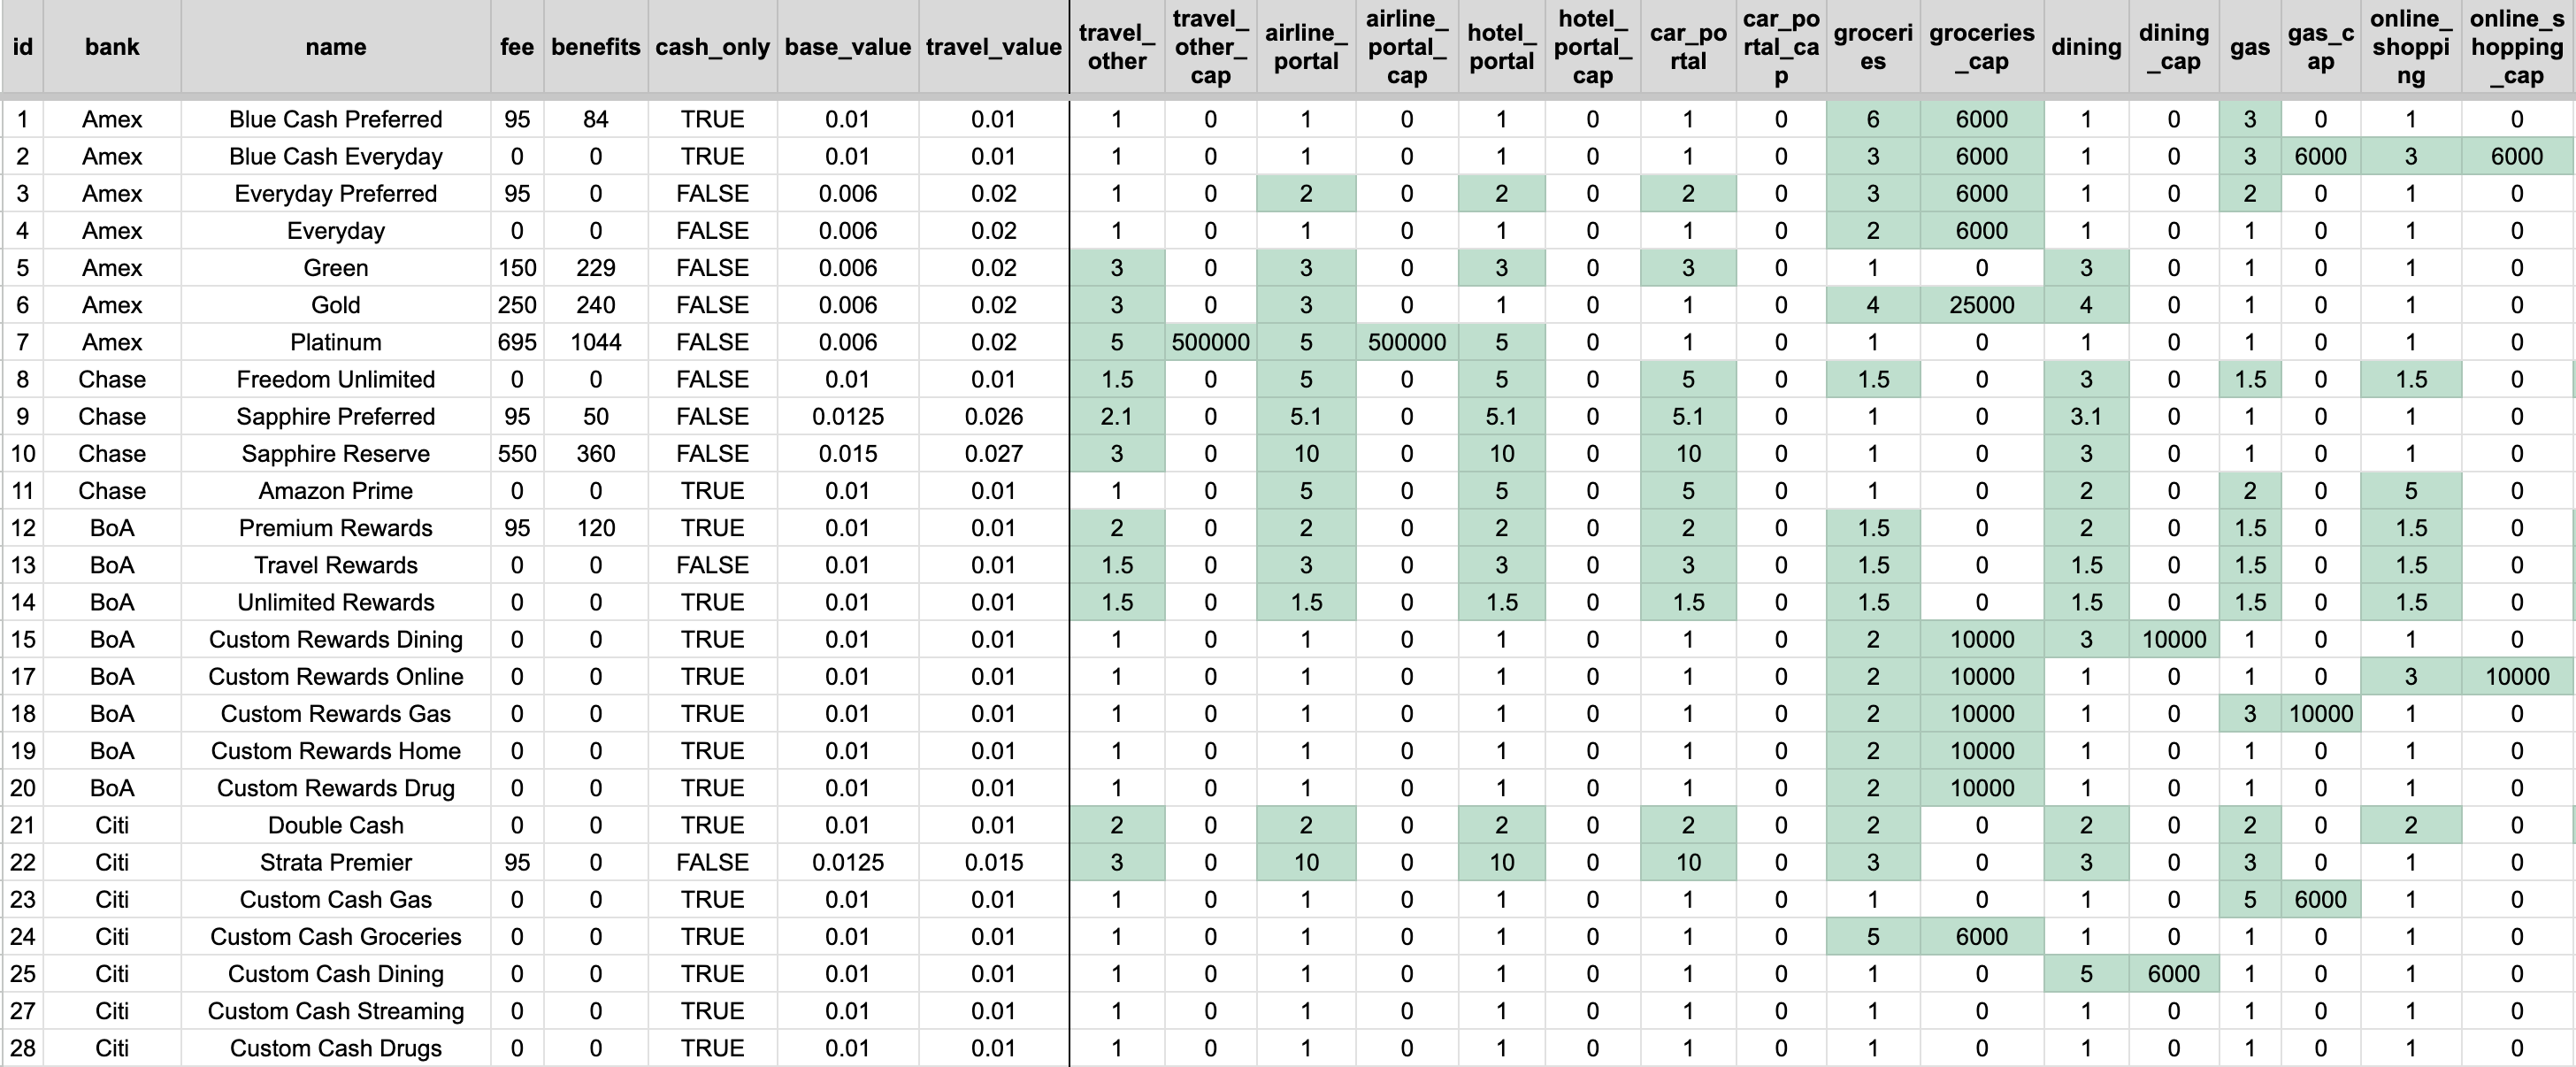
\includegraphics[width=1.0\textwidth]{../Misc/CreditCardTable.png}
    \end{center}    
\end{frame}    

\begin{frame}
    \frametitle{Users Data}
    \begin{itemize}
        \item Average budget (percentage per category) from BLS Consumer Expenditure Survey (2022)
        \item Corrected for non-credit card spend (rent, insurance, etc.)
    \end{itemize}
    \begin{columns}[c]
        \begin{column}{0.7\textwidth}
        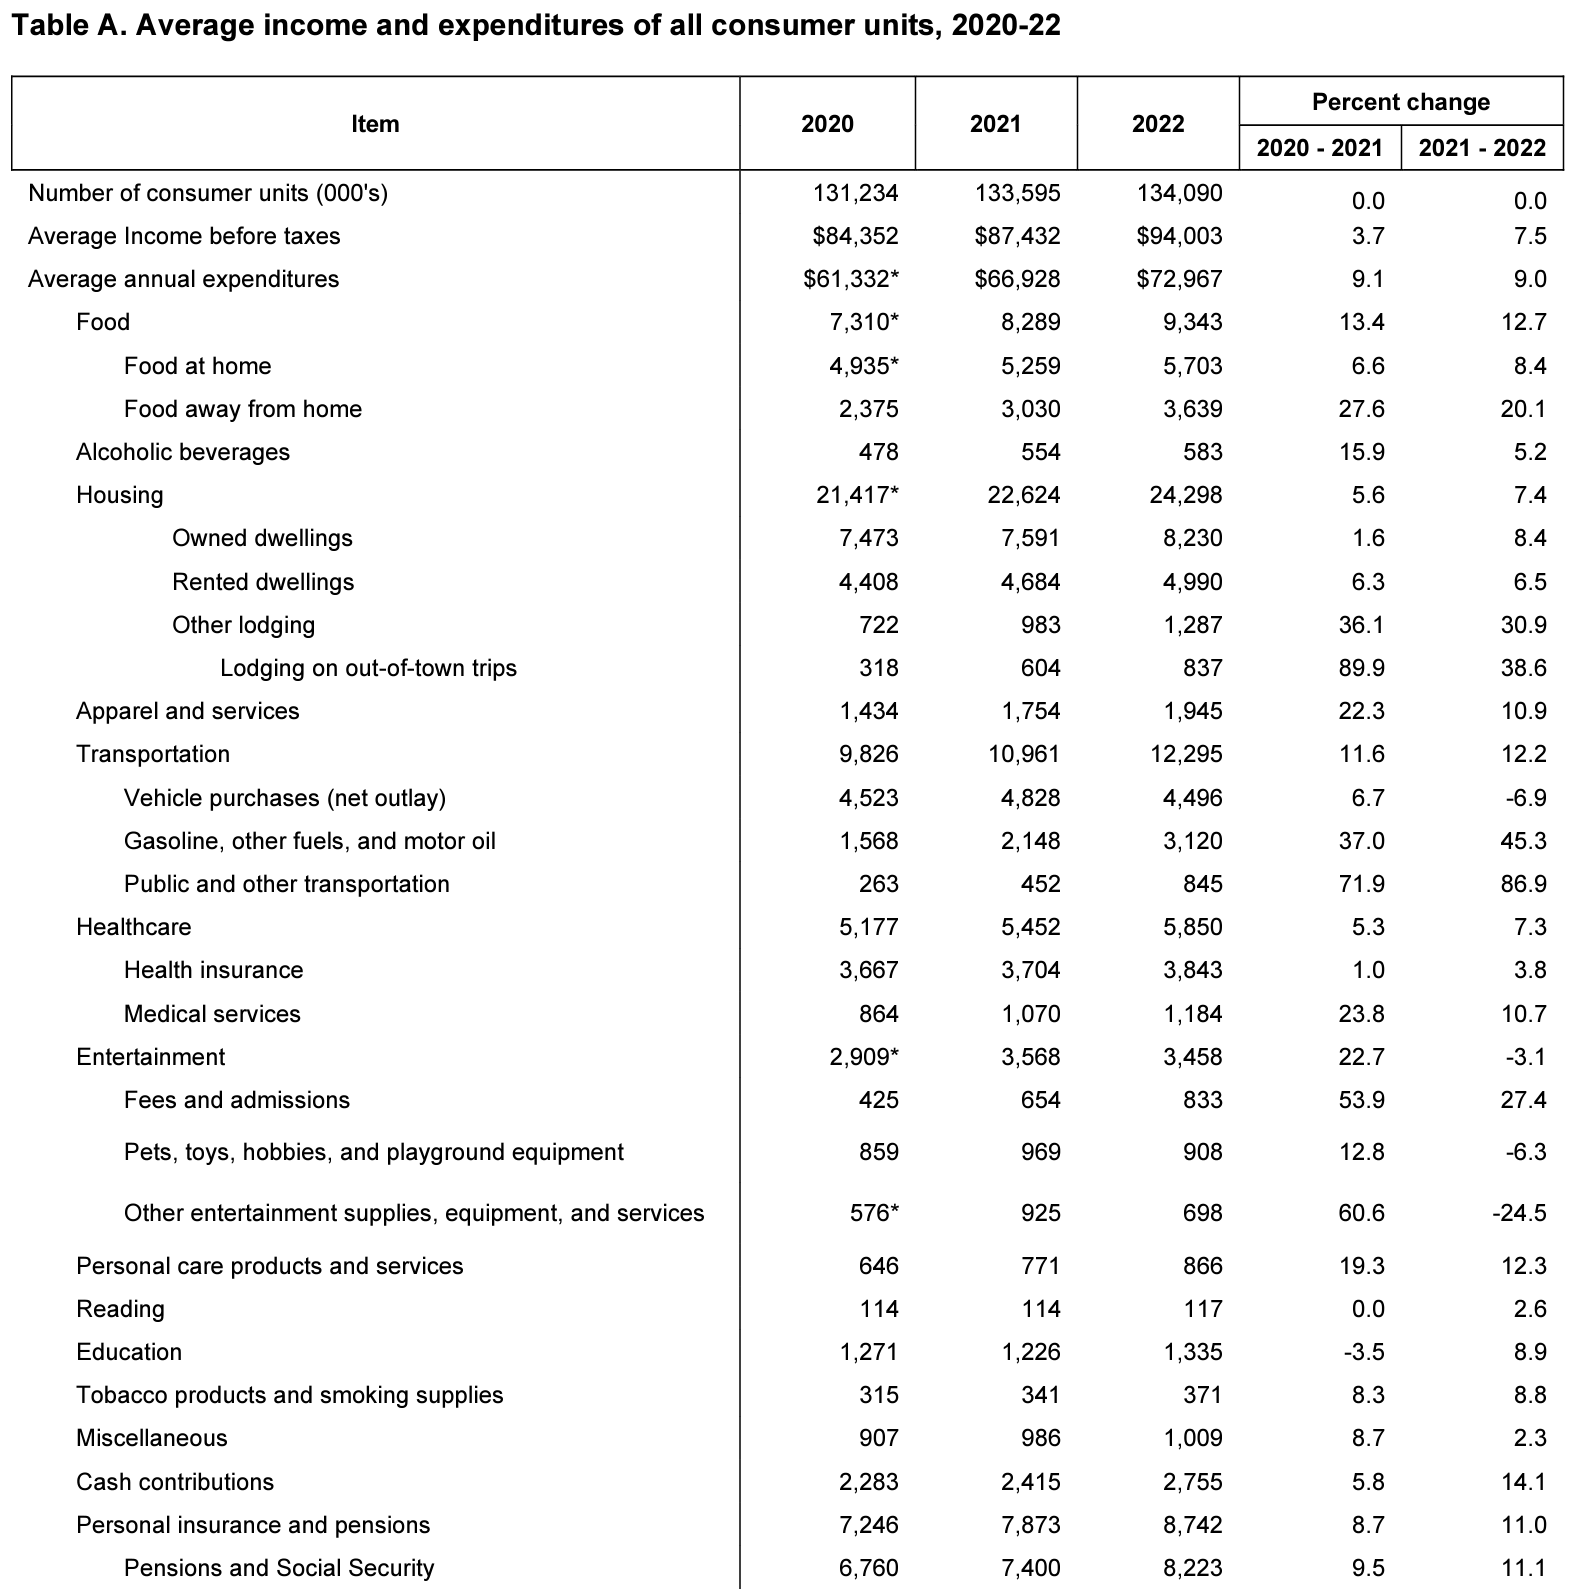
\includegraphics[width=0.95\textwidth]{../Misc/BLSTableA.png}
        \end{column}
        \begin{column}{0.3\textwidth}
        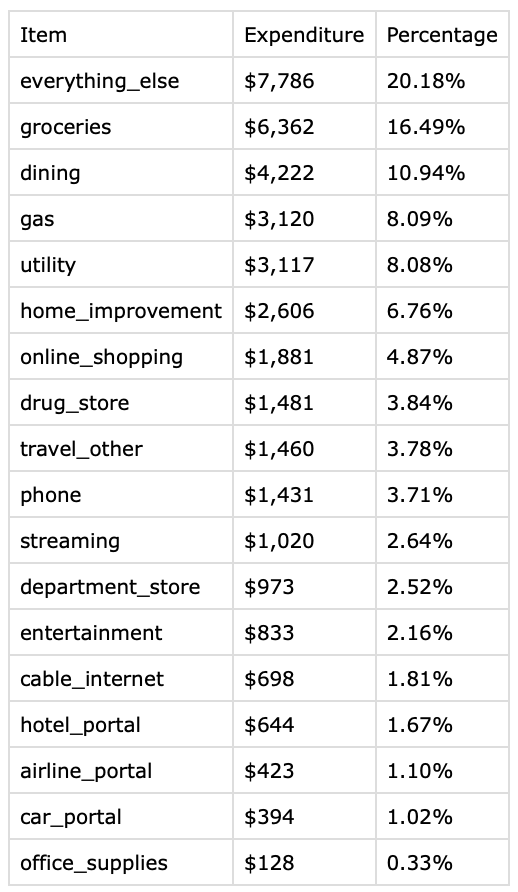
\includegraphics[width=1.0\textwidth]{../Misc/Budget.png}
        \end{column}
    \end{columns}
\end{frame}    

% FINAL SLIDE
\begin{frame}
    \frametitle{Using the Data for Simulations}
    \begin{itemize}
        \item First test if the algorithm works (Sensitivity Analysis)
        \begin{itemize}
        \item Assume low-vs-high income (e.g. \$50k vs \$150k)
        \item Assume spending 41\% on credit cards (BLS survey)
        \item Assume $\eta, \theta \; \in \; [0, 0.5, 1.0]$
        \item How does the net benefit change with these assumptions and number of cards?
        \end{itemize}
    \end{itemize}
    \bigskip
    \begin{itemize}
        \item If successful, attempt Monte-Carlo Simulations
        \begin{itemize}
        \item Sample income from log-normal distribution
        \item Sample $\eta, \theta$ from uniform distributions
        \end{itemize}
    \end{itemize}
\end{frame}    

\section{Summary \& Conclusions}

\begin{frame}
    \frametitle{Summary \& Conclusions}
    \begin{itemize}
        \item Financially sophisticated credit card users can benefit from inefficiencies in rewards programs by using the right credit cards
        \bigskip
        \item By using a Dynamic Program and Monte Carlo Simulations I aim to quantify this benefit for the average spending card user\\
        \bigskip
        \item Next week we'll talk more about the data!
    \end{itemize}
\end{frame}

% \begin{frame}
%     \frametitle{Summary \& Conclusions}
%     \begin{quote}
%         \centerline{Next week we'll talk more about the data!}
%         \vskip 16pt
%         \centerline{To Be Continued\ldots}
%     \end{quote}
% \end{frame}
    
    

\begin{frame}
    \frametitle{References}
    \bibliographystyle{../chicago}
    \bibliography{../References}
\end{frame}    


% NOTES:


% 1. Credit card rewards are a big industry. 
%     - give numbers on the bank profits
%     - give numbers on the total outstanding consumer credit card debt
%     - See CFPB report October 2023.

% 2. Notwithstanding all the debt, credit cards can also be rewarding.
%     - Explain the economics of credit card transactions.
%     - Interchange fees, processing fees, network fees. See Hayashi 2009!!!
%     - Retailers calculate this into all prices. If you pay cash or debit you subsidize the credit card users who get rewards (average $151 per year).
%     - Reverse Robinhood mechanism: low incomes subsidize high incomes, but this seems to be only partially true: it's mostly low FICO scores who subsidize high FICO scores.

% 3. Agarwal paper.
%     - The financially naive subsidize the financially sohphisticated.
%     - Financial sophistication is linked to FICO scores.
%     - Explain what FICO scores are and show the compisition that makes up the scores.
%     - Show a graph or two from their results.

% 4. How to become financially sophisticated.
%     - Optimal behavior
%     - How to increase your FICO score
%     - Show my own data that many cards don't tank your score permanently.
%     - And you don't need to revolve a balance for a good score!
%     - This should already benefit most consumers (don't make naive, sub-optimal decisions) and get them rewards instead of paying interest and fees.

% 5. Taking it to the next level.
%     - But how can we optimize this further? 
%     - I will study how to select the optimal credit card portfolio for maximum rewards.
%     - Comparing different heuristics? Optimal vs 1-card vs 
%       something-sub-optimal-most-people-tend-to-do?
%     - Do for different simulated budgets and look for heterogeneity across budgets or 
%       typical users.

% 6. Budgets
%     - Research average spending of americans and change it to 5 typical consumers?
%     - See CFPB Chapter 3! Maybe split consumers by FICO score that correlates with budget?

% 7. Very simple economic model
%     - Y = X*b + benefits - fees, etc.

% WARNING: be sure to keep material for presentation 2!!!
% Presentation 2 (June 17): Presentation of the outline paper, including data sources and how I plan to solve the problem using the data.



%\begin{appendix}
\section{Data Appendix}
\begin{frame}
\frametitle{Data Appendix}
\begin{itemize}

\item 1.
\item 2.
\item 3.

\end{itemize}
\end{frame}
\end{appendix}


\end{document}
